\documentclass{beamer}
\title{A Sociable Virus?\\
	A Comparison and Investigation of Reproducibility of
	Methods for Analysing COVID-19 Transmission Chains
	Using Graph Networks}
\author{Simon Westfechtel}
\date{03.08.2023}
\usetheme{Madrid}
\AtBeginSection[]
{
	\begin{frame}
		\frametitle{Table of Contents}
		\tableofcontents[currentsection]
	\end{frame}
}

\usepackage[absolute,overlay]{textpos}
\usepackage{graphicx}
\usepackage{tikz}
\usepackage{tabularx}
\usepackage{amsmath}
\usepackage{subcaption}
\usepackage[style=apa]{biblatex}
\addbibresource{sources.bib}

\DeclareMathOperator*{\argmax}{argmax}

\begin{document}
	\frame{\titlepage}
	
	\section{Introduction}
	
	\begin{frame}{Case contact networks}
		\begin{itemize}
			\item Many contact tracing initiatives during Covid-19
			\item Data records of general form $(time,source,contact)$
			\item Additional covariates depending on initiative
		\end{itemize}
	\end{frame}

	\begin{frame}{Case contact networks - illustration}
		\begin{figure}
				\centering
				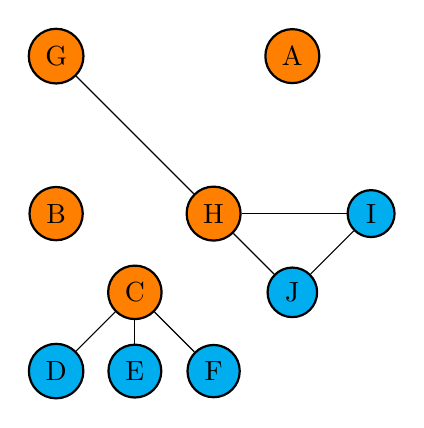
\begin{tikzpicture}
					\begin{scope}[every node/.style={circle,thick,draw,fill=orange}]
						\node (A) at (2,2) {A};
						\node (B) at (-1,0) {B};
						\node (G) at (-1,2) {G};
						\node (C) at (0,-1) {C};
						\node (H) at (1,0) {H};
					\end{scope}
					
					\begin{scope}[every node/.style={circle,thick,draw,fill=cyan}]
						\node (D) at (-1,-2) {D};
						\node (E) at (0,-2) {E};
						\node (F) at (1,-2) {F};
						\node (I) at (3,0) {I};
						\node (J) at (2,-1) {J};
					\end{scope}
					
					\begin{scope}
						\path (C) edge node {} (D);
						\path (C) edge node {} (E);
						\path (C) edge node {} (F);
						\path (G) edge node {} (H);
						\path (H) edge node {} (I);
						\path (H) edge node {} (J);
						\path (I) edge node {} (J);
					\end{scope}
				\end{tikzpicture}
				\caption{Exemplary case contact network. Confirmed cases are coloured orange, and reported contacts are coloured cyan. This network contains four connected components: $\{\{A\},\{B\},\{C,D,E,F\},\{G,H,I,J\}\}$}
				\label{fig:example_case_network}
		\end{figure}
	\end{frame}

	\begin{frame}{Case contact networks - example}
		\begin{figure}
			\includegraphics[width=\linewidth,height=.9\textheight]{figures/shaanxi.png}
		\end{figure}
	\end{frame}

	\begin{frame}{Motivation}
		\begin{itemize}
			\item Pandemic research often neglects societal aspect
			\item Computational Social Science offers wide array of tools 
			\item Question: which tools to use for which task?
		\end{itemize}
	\end{frame}

	\section{Previous Work}
	
	\begin{frame}{Static network models by Yang et al.\footnote{\cite{hainan_publication,shaanxi_publication,xian_publication}}}
		\begin{itemize}
			\item Applied social network analysis to four smaller-sized networks from China
			\item Computed centrality measures (degree, betweenness and pagerank) and connected components
			\item Primary findings:
			\begin{enumerate}
				\item Infections in clusters rather than in chains
				\item Networks generally sparse with a few very influential actors
			\end{enumerate}
		\end{itemize}
		
	\end{frame}

	\begin{frame}{Limitations of static network models}
		\begin{itemize}
			\item No consideration given to time (all interactions are assumed to happen simultaneously)
			\item Limited insights into dynamics of interactions between actors
		\end{itemize}
	\end{frame}

	\begin{frame}{Relational hyperevent models by H\^ancean et al.\footnote{\cite{hancean2021role,hancean2022occupations}}}
		\begin{itemize}
			\item Applied relational hyperevent models to larger-sized network from Romania
			\item Investigated impact of 
			\begin{itemize}
				\item actor covariates (e.g. age)
				\item interaction dynamics (e.g. reciprocation)
			\end{itemize}
			on contact nomination likelihood
		\end{itemize}
	\end{frame}

	\begin{frame}{Primary findings}
		\begin{itemize}
			\item Positive cases are more likely to be older and female
			\item Age and sex homophily
			\item Tendency for reciprocation of contact nominations
			\item Tendency for co-nominees to interact with each other
			\item Being nominated as a contact increases likelihood of testing positive
			\item Being tested positive increases likelihood of being nominated as a contact
		\end{itemize}
	\end{frame}
	
	\section{Methodology}
	
	\begin{frame}{Social network analysis}
		\begin{itemize}
			\item Based on graph theory
			\item $G = (V,E)$, where $V$ is the set of actors (cases and contacts), and $E$ is the set of interactions (contact nominations)
		\end{itemize}
	\end{frame}

	\begin{frame}{Social network analysis}
		Computed statistics:
		\begin{itemize}
			\item Degree centrality\footnote{\cite{golbeck}}: $C_D(v) = \frac{\text{deg}(v)}{\lvert V \rvert - 1}$
			\item Betweenness centrality\footnote{\cite{golbeck}}: $C_B(v) = \sum_{s\neq v\neq t\in V}\frac{\sigma_{st}(v)}{\sigma_{st}}$
			\item Pagerank centrality\footnote{\cite{gleich_pagerank}}: $C_P(v) = \sum_{u \in B_v}\frac{C_P(u)}{\text{deg}(u)}$
			\item Average shortest path length
			\item Component size
		\end{itemize}
	\end{frame}

	\begin{frame}{Social network analysis}
		Computed network statistics and actor covariates (nominator, nominee, difference) were combined into an ordinary least-squares regression model, conditioned on contact nomination between two actors
	\end{frame}

	\begin{frame}{Relational event models}
		\begin{itemize}
			\item Statistical models used for analysing ordered sequences of interactions among actors
			\item Take timing of events into consideration
			\item Use order and timing to make inferences about dynamics of interactions
		\end{itemize}
	\end{frame}

	\begin{frame}{Relational event models}
		Model probability of an event sequence $E$:
		\begin{equation*}
			P(E) = \prod_{i=1}^{n}P(e_i|E_{<t_i})
		\end{equation*}
		Partial likelihood of a particular event:
		\begin{equation*}
			P(e_i|E_{<t_i};\theta) = \frac{\lambda(u_i,v_i,t_i;\theta)}{\sum_{uv\in R_{t_i}}\lambda(u,v,t_i;\theta)}
		\end{equation*}
		Hazard rate of dyad:
		\begin{align*}
			\lambda(u,v,t_i;\theta) &= \lambda_0(t_i) \cdot \lambda_1(u,v,t_i;\theta)\\
			\lambda_1(u,v,t_i;\theta) &= \exp(\theta^T s(u,v;E_{<t_i}))\\
			&= \exp(\sum_h \theta_h \cdot s_h(u,v;E_{<t_i}))&&
		\end{align*}\footnote{\cite{butts20084,pilny_rem,stadtfeld2017interactions}}
	\end{frame}

	\begin{frame}{Relational event models}
		Model parameters are estimated through maximum likelihood estimation:
		\begin{equation*}
			\hat{\theta} = \argmax_{\theta} P(E|\theta)
		\end{equation*}
		Here: Cox proportional hazards model with case-control sampling; includes actor covariates (nominator, nominee, difference) and network statistics.
	\end{frame}

	\begin{frame}{Relational event models}
		Network statistics:
		\begin{itemize}
			\item Nomination activity: \[nomination.activity(e(u,v,t_i)) = \sum_{v' \in V} e(u,v',<t_i)\]
			\item Exact repetition: \[exact.repetition(e(u,v,t_i)) = \sum e(u,v,<t_i)\]
			\item Reciprocation: \[reciprocation(e(u,v,t_i)) = \sum_{u' \in U} e(u',u,<t_i)\]
			\item Exact reciprocation: \[exact.reciprocation(e(u,v,t_i)) = \sum e(v,u,<t_i)\]
		\end{itemize}
	\end{frame}

	\begin{frame}{Relational event models}
		\begin{itemize}
			\item Transitive tie: \[transitive.tie(e(u,v,t_i)) = \sum_{x=1}^{\lvert \mathcal{R} \rvert} \min [d(u,x,A_{t_i}), d(x,v,A_{t_i})]\]
			\item Cyclical tie: \[cyclical.tie(e(u,v,t_i)) = \sum_{x=1}^{\lvert \mathcal{R} \rvert} \min [d(v,x,A_{t_i}), d(x,u,A_{t_i})]\]
			\item Shared source: \[shared.source(e(u,v,t_i)) = \sum_{x=1}^{\lvert \mathcal{R} \rvert} \min [d(x,u,A_{t_i}), d(x,v,A_{t_i})]\]
			\item Shared target: \[shared.target(e(u,v,t_i)) = \sum_{x=1}^{\lvert \mathcal{R} \rvert} \min [d(u,x,A_{t_i}), d(v,x,A_{t_i})]\]\footnote{\cite{butts20084,pilny_rem,brandes2009networks,perry2013point}}
		\end{itemize}
	\end{frame}

	\begin{frame}{Relational event models}
		Limitation: Interactions are assumed to be dyadic
	\end{frame}

	\begin{frame}{Relational hyperevent models\footnote{\cite{perry2013point,lerner2019rem,lerner2021relational}}}
		\begin{itemize}
			\item Based on REM
			\item New: polyadic hyperevents instead of dyadic events $\rightarrow$ uses hypergraphs
			\item Previously: event $e_i(u,v,t_i)$
			\item Now: hyperevent $e_i(h_i,t_i);\: h_i = (\mathcal{U},\mathcal{V})$
			\item Special case here: $\lvert \mathcal{U} \rvert = 1$
		\end{itemize}
	\end{frame}

	\begin{frame}{Relational hyperevent models}
		Definition of statistics changes slightly compared to REM:
		\begin{itemize}
			\item Actor covariates: nominator, nominee set average, difference between nominator and nominee set, and variance among nominees
			\item Network effects: repetition on partial subsets and in differing order
			\item In general: adjustment to nature of hyperedges
		\end{itemize}
	\end{frame}

	\begin{frame}{Relational hyperevent models}
		Example for changed definition of statistics (exact reciprocation):
		\begin{figure}
			\centering
			\begin{subfigure}[t]{0.4\linewidth}
				\vskip 0pt
				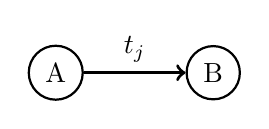
\begin{tikzpicture}
					\begin{scope}[every node/.style={circle,thick,draw}]
						\node (A) at (0,0) {A};
						\node (B) at (2,0) {B};
					\end{scope}
					
					\begin{scope}[every edge/.style={draw=black,very thick}]
						\path [->] (A) edge node [above] {$t_j$} (B);
					\end{scope}
				\end{tikzpicture}
			\end{subfigure}
			\hfill
			\begin{subfigure}[t]{0.4\linewidth}
				\vskip 0pt
				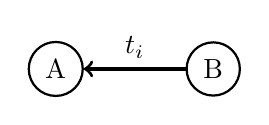
\begin{tikzpicture}
					\begin{scope}[every node/.style={circle,thick,draw}]
						\node (A) at (0,0) {A};
						\node (B) at (2,0) {B};
					\end{scope}
				
					\begin{scope}[every edge/.style={draw=black,very thick}]
						\path [->] (B) edge node [above] {$t_i$} (A);
					\end{scope}
				\end{tikzpicture}
			\end{subfigure}
			\caption{Exact reciprocation in REM. $t_j < t_i$}
		\end{figure}
		
		
		\begin{figure}
				\centering
				\begin{subfigure}[t]{0.4\linewidth}
					\vskip 0pt
					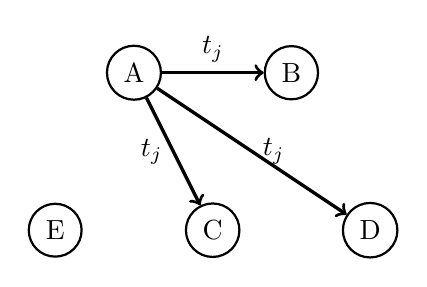
\begin{tikzpicture}
						\begin{scope}[every node/.style={circle,thick,draw}]
							\node (A) at (0,2) {A};
							\node (B) at (2,2) {B};
							\node (C) at (1,0) {C};
							\node (D) at (3,0) {D};
							\node (E) at (-1,0) {E};
						\end{scope}
						
						\begin{scope}[every edge/.style={draw=black,very thick}]
							\path [->] (A) edge node [above] {$t_j$} (B);
							\path [->] (A) edge node [left] {$t_j$} (C);
							\path [->] (A) edge node [right] {$t_j$} (D);
						\end{scope}
					\end{tikzpicture}
				\end{subfigure}
				\hfill
				\begin{subfigure}[t]{0.4\linewidth}
					\vskip 0pt
					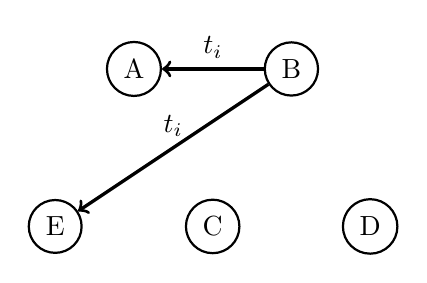
\begin{tikzpicture}
						\begin{scope}[every node/.style={circle,thick,draw}]
							\node (A) at (0,2) {A};
							\node (B) at (2,2) {B};
							\node (C) at (1,0) {C};
							\node (D) at (3,0) {D};
							\node (E) at (-1,0) {E};
						\end{scope}
						
						\begin{scope}[every edge/.style={draw=black,very thick}]
							\path [->] (B) edge node [above] {$t_i$} (A);
							\path [->] (B) edge node [above] {$t_i$} (E);
						\end{scope}
					\end{tikzpicture}
				\end{subfigure}
				\caption{Exact reciprocation in RHEM. $t_j < t_i$}
		\end{figure}
	\end{frame}

	\begin{frame}{Relational hyperevent models}
		Example for new statistic (partial repetition):
		\begin{figure}
				\centering
				\begin{subfigure}[t]{0.45\linewidth}
					\vskip 0pt
					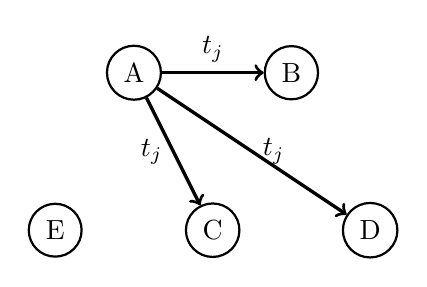
\begin{tikzpicture}
						\begin{scope}[every node/.style={circle,thick,draw}]
							\node (A) at (0,2) {A};
							\node (B) at (2,2) {B};
							\node (C) at (1,0) {C};
							\node (D) at (3,0) {D};
							\node (E) at (-1,0) {E};
						\end{scope}
						
						\begin{scope}[every edge/.style={draw=black,very thick}]
							\path [->] (A) edge node [above] {$t_j$} (B);
							\path [->] (A) edge node [left] {$t_j$} (C);
							\path [->] (A) edge node [right] {$t_j$} (D);
						\end{scope}
					\end{tikzpicture}
					\caption{Event $(A,\{B,C,D\},t_j)$}
				\end{subfigure}
				\hfill
				\begin{subfigure}[t]{0.45\linewidth}
					\vskip 0pt
					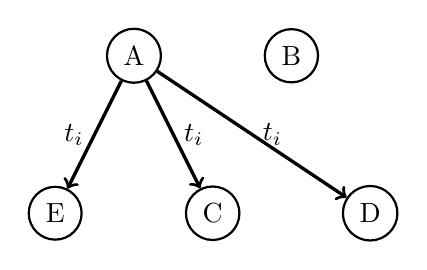
\begin{tikzpicture}
						\begin{scope}[every node/.style={circle,thick,draw}]
							\node (A) at (0,2) {A};
							\node (B) at (2,2) {B};
							\node (C) at (1,0) {C};
							\node (D) at (3,0) {D};
							\node (E) at (-1,0) {E};
						\end{scope}
						
						\begin{scope}[every edge/.style={draw=black,very thick}]
							\path [->] (A) edge node [right] {$t_i$} (C);
							\path [->] (A) edge node [right] {$t_i$} (D);
							\path [->] (A) edge node [left] {$t_i$} (E);
						\end{scope}
					\end{tikzpicture}
					\caption{Event $(A,\{C,D,E\},t_i)$}
				\end{subfigure}
				\caption{Illustration of partial repetition in relational hyperevent models. Time ordering is $t_j < t_i$.}
		\end{figure}
	\end{frame}

	\begin{frame}{Relational hyperevent models}
		Model parameters are likewise estimated using Cox proportional hazards models with case-control sampling.
	\end{frame}
	
	\section{Results and Discussion}
	
	\begin{frame}{Reproducibility}
		\begin{itemize}
			\item Results produced by SNA were in full agreement with works by Yang et al.
			\item Results produced by RHEM were in partial agreement with works by H\^ancean et al.:
			\begin{itemize}
				\item Network effects were reproducible
				\item Effects of actor covariates were not
				\item Most probable reason: difference in dataset size
			\end{itemize}
		\end{itemize}
	\end{frame}

	\begin{frame}{SNA findings}
		\begin{itemize}
			\item ANOVA: significant differences between regions w.r.t. degree centrality, pagerank centrality and shortest path length
			\item Negative correlation between network size and density
			\item Infections happen in clusters isolated from the larger network, rather than in chains
			\item Actor age largely has no significant and/or consistent effect in most networks
			\item Bias towards males for nominator and nominee roles in all networks except Romania (female bias)
			\item Sex heterophily in all networks except Romania (homophily)
		\end{itemize}
	\end{frame}

	\begin{frame}{REM findings}
		\begin{itemize}
			\item Positive effects for general and exact reciprocation in most networks
			\item Positive effects for shared source and cyclical tie in most networks
			\item Nominator and nominee tend to be younger and of a similar age (age homophily)
			\item Nominator and nominee tend to be of different sex (sex heterophily)
		\end{itemize}
	\end{frame}

	\begin{frame}{RHEM findings}
		Results of RHEM are mostly in agreement with those of REM
	\end{frame}

	\begin{frame}{Model fit}
		\begin{itemize}
			\item Computed $R^2$ values show that static network models have best model fit
			\item REM and RHEM perform especially poorly on small networks
		\end{itemize}
	\end{frame}

	\begin{frame}{Main takeaways}
		\begin{itemize}
			\item SNA and REM/RHEM should be used for different tasks
			\item Actor covariates play a mostly consistent and significant role across different regions
			\item Age homophily, sex heterophily
			\item Nominations mostly among actors with the same place of residence
			\item Nominations mostly among family members
			\item Lower chance for medical workers to act as either nominator or nominee
		\end{itemize}
	\end{frame}

	\begin{frame}{Main takeaways}
		\begin{itemize}
			\item Contact nominations occur in isolated clusters
			\item Contact nominations tend to be reciprocated
			\item Contact nominations increase chance for interaction between nominees
			\item Tendency for nominations to go around in circles
			\item Repeated interactions are rare
			\item Discrepancies between results of REM and RHEM in some instances suggest existence of higher-order effects $\rightarrow$ give credence to the usage of RHEM
		\end{itemize}
	\end{frame}
	
	\section{Outlook}
	
	\begin{frame}{What's next}
		\begin{itemize}
			\item Divide models into sub-models for actor covariates and network effects
			\item Apply to a network that covers a longer timespan
			\item Investigate other network effects
		\end{itemize}
	\end{frame}
	
	\begin{frame}[allowframebreaks]
		\frametitle{Bibliography}	
		\printbibliography
	\end{frame}
\end{document}